\documentclass[letterpaper]{article}

% AAAI header
\usepackage{aaai} 
\usepackage{times} 
\usepackage{helvet} 
\usepackage{courier}
\usepackage{url}

% fancy symbols
\usepackage{amsmath}
\usepackage{amsthm}
\usepackage{amssymb}
% \usepackage{natbib}
\usepackage{graphicx}

\newtheorem{thm}{Theorem}
\newtheorem{lemma}{Lemma}
\newtheorem{definition}{Definition}
\newtheorem{question}{Question}

\title{Classifying reviews}
\author{Ertan Dogrultan \and Cesar Romero \and Paul Wais\\
Computer Science Department \\
University of California, Los Angeles\\
Los Angeles, California 90095\\
\texttt{\{ertan,romero\}@cs.ucla.edu, pwais@ucla.edu}}

\begin{document}
\maketitle{}
\begin{abstract}
  We have an awesome translator that works for amazon and yelp reviews.
\end{abstract}

\section{Introduction}
\label{sec:introduction}

We tell a story to motivate the problem. We mention Jenn's
work~\cite{JennLearnDiffDomains} and the sentiment classification
work~\cite{PangSentimentClassification}.

\section{Domain Adaptation}
\label{sec:background}

\emph{Here, we explain what domain adaptation is and its important
prameters.}
We are interested in being able to classify reviews in general - not
just from a specific source or category. A natural problem to consider
is Domain Adaptation. In this setting, there is a source domain $S$
and a target domain $T$. The goal is to be able to classify reviews in
$T$ when most of our data comes from $S$. 

Include the fancy Theorem here that will be used to predict the error
of the calssifiers in the domain adaptation setting.

\subsection{$\alpha$-error}
\label{sec:alpha-error}

Explain the $\alpha$-error here.

\subsection{Estimating the distance}
\label{sec:estimating-distance}

We train a linear classifier to learn to which domain a review
belongs. The error of this classifier is used as an estimate of the
distance between the distributions.

\section{Mid-quarter report}
\label{sec:mid-quarter-report}

In the report we cited~\cite{citeulike:352583} among others. Figure~

\begin{figure*}[h]
  \centering
  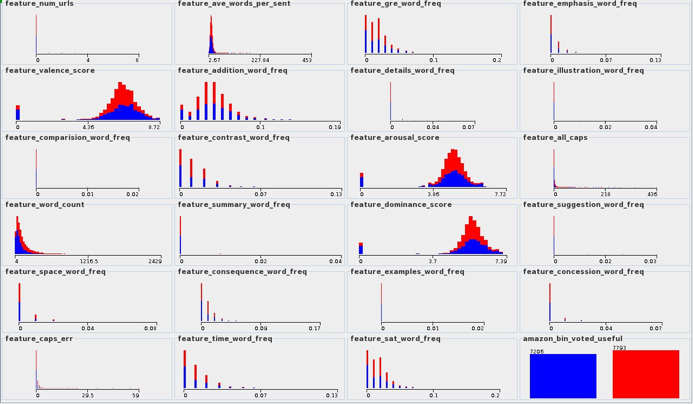
\includegraphics[scale=.5]{features_distributions}
  \caption{This is the figure from the report}
  \label{fig:dist}
\end{figure*}

\section{Features}
\label{sec:features}

A concise and example-driven description of all our features.  This
will probably take a little while to write :). And we should probably
have a reference to ANEW~\cite{DoddsANEWPaper}.

Link to our github:
\url{https://github.com/pwais/thumbsup}

\section{Experiments}
\label{sec:experiments}

We present two sets of experiments. In the first set, we use different
models to learn the quality of the review using the features described
in~\ref{sec:features}. Then, we use the model that performs best in
the first set of experiments to classify reviews in a domain
adaptation setting. We use the WEKA machine learning suite for our
experiments~\cite{weka}.

\subsection{Learning Reviews}
\label{sec:learning-reviews}

We use three different models to learn the quality of the reviews:
Support Vector MAchines (SVMs), Adaboost, and Naive Bayes.

\emph{Our original data includes a lot of noise. We can probably talk
  here about taking only the extreme cases: either very good (over
  85th percentile) or very bad (under 5th percentile).}

\subsection{Domain Adaptation}
\label{sec:domain-adaptation}

In this set of experiments we use the \emph{insert model here} to
learn from both domains. For this experiments, Yelp is considered to be
the \emph{target} and Amazon the \emph{source}.

We estimate the distance between the distributions, $\zeta$ , using the metod
previously explained in the domain adaptation Section. For the first
set of domain adaptation experimentes, we vary the value of $\beta \in
\{0.1, 0.2, 0.4, 0.8\}$ while holding $\zeta$ constant.

Using a fixed $\beta$ we want see how well the classifier performs
when the distance between the target and source distribution
varies. To alter $\zeta$, we consider only a specific category on each
domain. From the source domain (Amazon), we consider the set of
categories $C_S=\{$ Books, Electronics, DVDs and Clothing\}. From the
target domain (Yelp) we consider only one category
$C_T=$\{Restaurants\}. For each combination in $C_s\times C_T$ we train
and test a different classifier. Notice that, to estimate the distance
between any of the two categories in the four possible combinations,
we need to train a separate linear classifier to estimate the distance
as we did before. Figure~\ref{fig:domain-adaptation} shows the errors
of these classifiers together with their theoretical bounds.

\begin{figure}
  \centering
  
  \caption{Domain Adaptation Experiments}
  \label{fig:domain-adaptation}
\end{figure}

\section{Citations to use}
Jenn's domain adaption paper \cite{JennLearnDiffDomains}\\
ANEW paper \cite{DoddsANEWPaper}\\
Pang et al sentiment classification \cite{PangSentimentClassification}\\
The WEKA paper that they ask users to cite \cite{weka} \\

\bibliography{bib}
\bibliographystyle{aaai}

\end{document}
